\documentclass[12pt, letterpaper]{article}
\usepackage{graphicx}
\usepackage[T1]{fontenc}
\usepackage[polish]{babel}
\usepackage[utf8]{inputenc}

\graphicspath{{images/}}

%--------------------------------------------------------------------------------------------------
%       TITLE SECTION
%--------------------------------------------------------------------------------------------------
\begin{titlepage}
 

\includegraphics[scale=0.2]{ur_inf_logo}\\ \\ \\ \\

\begin{center}
	{ \huge \bfseries Programowanie obiektowe}\\[0.4cm] 

	\textsc{\Large Aplikacja bankowa}\\[0.5cm] \\ \\ \\ \\ 
	
	\vspace{0.8cm}	
	
	\emph{Autorzy:} \\
	\textbf{Oskar Paśko} (117987)\\
	\textbf{Eliza Tworkowska} (119003)	
	
	
	\vspace{0.8cm}
	
	\emph{Kierunek:} \\
	Informatyka i ekonometria
	
	\vspace{8cm}
	
	\emph{Prowadzący:} \\
	mgr inż. Ewa Żesławska\\ \\ \\ \\ 
	
	\vspace{2cm}
	
	Rzeszów, 2023
\end{center}
\end{titlepage}
%--------------------------------------------------------------------------------------------------
%      END TITLE SECTION
%--------------------------------------------------------------------------------------------------

\begin{document}
\newpage

%--------------------------------------------------------------------------------------------------
%      SPIS TREŚCI
%--------------------------------------------------------------------------------------------------
\tableofcontents

\newpage

%--------------------------------------------------------------------------------------------------
%      OPIS ZAŁOŻEŃ
%--------------------------------------------------------------------------------------------------
\section{Opis założeń projektu}

\quad Niniejszy projekt dotyczy aplikacji bankowej, która ma za zadanie ułatwić klientowi
z korzystania z dostępnych na rynku usług bankowych.

\quad Użytkownik posiadający konto w bazie danych niniejszej aplikacji może się zalogować do niej za pomocą swojego numeru klienta oraz hasła. Na głównej stronie może sprawdzić swoje aktualne saldo, na które składają sie salda wszystkich jego kart posiadanych w banku. Tabela ze wszystkimi kartami widoczna jest w centralnym punkcie strony głównej. Dodatkowo, na stronie głównej, użytkownik może sprawdzić historię transakcji. Ponadto klient może dokonać wpłaty na wybraną przez siebie kartę oraz wypłaty z wybranej przez siebie karty z założeniem, że posiada na niej wystarczającą ilość środków. Dzięki aplikacji możliwe jest również dokonanie przelewów z założeniami takimi 
jak w przypadku wpłat i wypłat. Użytkownik ponadto może dodać nową kartę płatniczą lub usunąć isniejącą przy 
założeniu,że jej bilans wynosi 0 zł.

\newpage

%--------------------------------------------------------------------------------------------------
%      SPECYFIKACJA WYMAGAŃ
%--------------------------------------------------------------------------------------------------
\section{Specyfikacja wymagań}

\subsection{Wymagania funkcjonalne}
\begin{itemize}
\item Aplikacja oferuje połączenie z bazą danych.
\item Bank oferuje usługi użytkownikom zarejestrowanym w aplikacji.
\item Bank oferuje możliwość zarejestrowania się nowym użytkownikom.
\item Klient może wpłacić lub wypłacić pieniądze z wybranej karty.
\item Klient może dokonać przelewu na wybraną kartę.
\item Klient może sprawdzić saldo swoich kart płatniczych.
\item Klient może sprawdzić historię przelewów.
\item Zarejestrowany klient może dodać nową kartę płatniczą do swojego konta.
\end{itemize}


\subsection{Wymagania niefunkcjonalne}
\begin{itemize}
\item Możliwość dodawania, usuwania oraz edycji rekordów w bazie podczas działania aplikacji.
\item Aplikacja jest przyjazna dla klienta i jego rodziny oraz jest prosta\\ w użyciu.
\item Aplikacja tworzona jest w języku Java.
\item Aplikacja nawiązuje połączenie z bazą danych w języku MySQL i używa rekordów w niej zapisanych.
\end{itemize}

\newpage

%--------------------------------------------------------------------------------------------------
%      OPIS TECHNICZNY BAZY DANYCH
%--------------------------------------------------------------------------------------------------
\section{Opis techniczny bazy danych}

\subsection{Opis założeń}

\quad Baza danych przechowuje dane klientów oraz należących do nich kart płatniczych, jak również  
historię wykonanych przelewów.\\

\quad Podczas działania aplikacji na bazie danych zostają wykonywane działania wyświetlania, modyfikowania, wstawiania oraz usuwania danych.

\subsection{Diagram ERD}

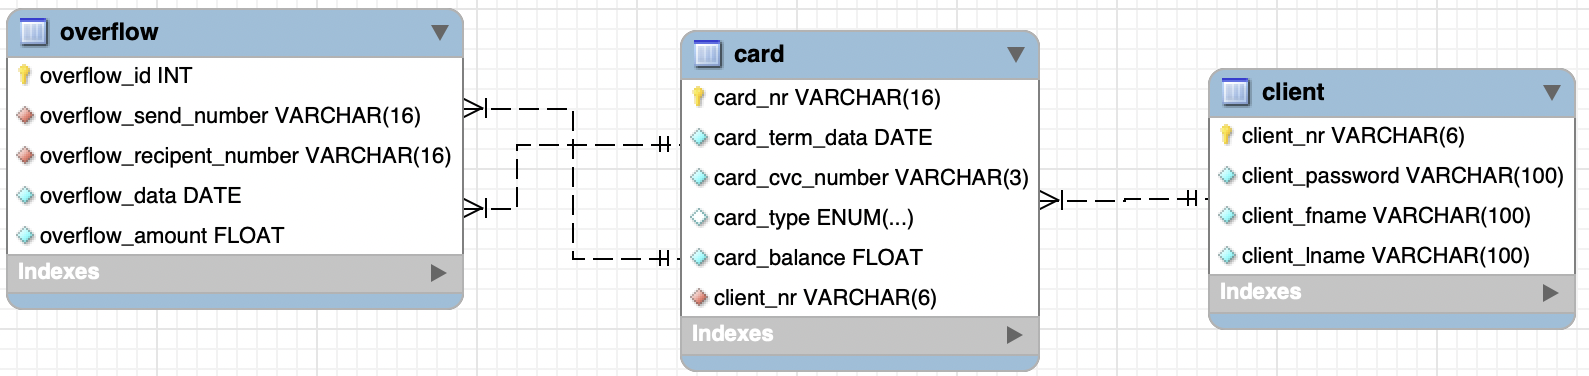
\includegraphics[scale=0.5]{erd}

\subsection{Opis tabel w bazie danych}

\subsubsection{Tabela client}

\quad Tabela "client" przechowuje informacje na temat klienta. Przechowywane informacje to sześciocyfrowy numer klienta, który jest kluczem głównym tabeli, hasło klienta oraz imię i nazwisko klienta.\\


\subsubsection{Tabela card}

\quad Tabela "card" przechowuje informacje o kartach płatniczych klientów.\\ W tabeli przechowujemy informacje o szesnastocyfrowym numerze karty, który pełni rolę klucza głównego, datę ważności karty, numer zabezpieczający cvc, który jest zawsze trzycyfrowy, typ karty, saldo znajdujące się na karcie oraz numer klienta posiadającego daną kartę. Numer ten jest zapisany jako klucz obcy tabeli połączony metodą wiele do jednego z tabelą "client".



\subsubsection{Tabela overflow}

\quad Tabela "card"  przechowuje informacje o przelewach dokonanych przez klienta. W tabeli przechowujemy klucz główny tabeli, numer karty, z której został wysłany przelew oraz numer karty, 
na którą został wysłany przelew. Dodatkowo przechowuje datę wykonania przelewu oraz jego wartość.

\newpage

%--------------------------------------------------------------------------------------------------
%       Warstwa użytkowa projektu
%--------------------------------------------------------------------------------------------------

\section{Warstwa użytkowa projektu}

\subsection{Diagram przypadków użycia}

\begin{center}
	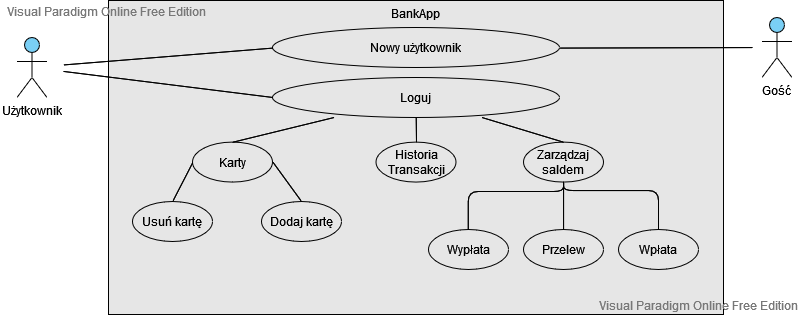
\includegraphics[scale=0.5]{UseCase}
\end{center}

\newpage

\subsection{LoginFrame}
\quad Po uruchomieniu aplikacji otwiera się okienko Logowanie, które umożliwia użytkownikowi:

\begin{itemize}
\item Zalogowanie się,
\item Zarejestrowanie się
\end{itemize}

\quad Okno logowanie łączy się z bazą danych za pomocą SQL i JDBC, dzięki czemu weryfikuje wprowadzone dane i wyświetla komunikaty zależne od wprowadzonych informacji. Jeśli walidacja danych przejdzie pomyślnie (to jest, login i hasło pokrywają się z użytkownikiem zawartym w bazie), aplikacja przechodzi do głównego widoku. Jeśli hasło lub login okaże się błędne, aplikacja wyświetli okno dialogowe informujące użytkownika o tym. Jeśli nastąpią błędy z połączeniem wyświetlą się okna dialogowe, które informują o tym. 
Jeśli użytkownik nie posiada dostępu do konta, może stworzyć nowe konto poprzez kliknięcie przycisku: “New User”\\

\begin{center}
	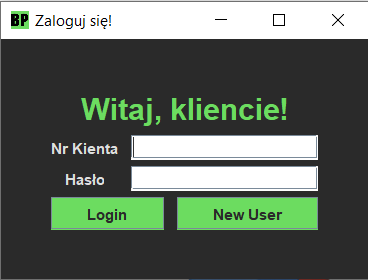
\includegraphics[scale=0.8]{login}
\end{center}

\newpage

\subsection{NewUser}
\quad Po kliknięciu przycisku w logowaniu “New User”, wyświetla się nowe okno umożliwiające stworzenie nowego użytkownika.
Okno NewUser to formularz składający się z następujących elementów: 

\begin{itemize}
\item Przycisk powracający, który wraca do okienka logowania
\item Pole do wprowadzenia nr klienta,
\item Pole do wprowadzenia hasła,
\item Pole do wprowadzenia imienia,
\item Pole do wprowadzenia nazwiska,
\item Przycisk "OK"
\end{itemize}

\quad Użytkownik może stworzyć nowego użytkownika po wprowadzeniu tych danych i aplikacja akceptuje je, jeśli się zgadzają z naszym formatem tworzenia użytkownika. Wymagania to:

\begin{itemize}
\item Wszystkie pola muszą mieć wprowadzoną wartość,
\item Nr klienta musi składać się tylko z liczb i być długości 6 cyfr,
\item Imie i nazwisko muszą składać się tylko z liter
\end{itemize}

\begin{center}
	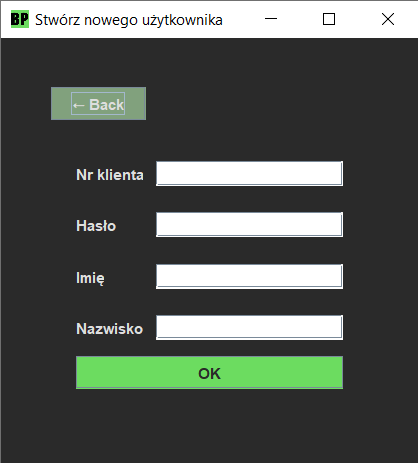
\includegraphics[scale=0.6]{newuser}
\end{center}

\quad Jeśli weryfikacja danych przejdzie pomyślnie, użytkownik doda nowe konto do bazy danych, a następnie zostanie z powrotem przeniesiony do okna logowania.
Jeśli użytkownik spróbuje stworzyć nowe konto, bez spełnienia wymagań, zostanie poinformowany o błędnych danych za pomocą okna dialogowego.
Jeśli użytkownik kliknie przycisk powrotu, zostanie przeniesiony na okno logowania bez utworzenia nowego konta.

\newpage

\subsection{MainFrame}

\quad Po pomyślnym zalogowaniu otworzy się główne okno aplikacji. 
W górnej części aplikacji znajduje się: 

\begin{itemize}
\item Przywitanie użytkownika imieniem znajdującym się w bazie danych,
\item Jego ogólne saldo (zsumowanie balansu wszystkich jego kart),
\item Przycisk wyloguj, który powraca nas do okna logowania,
\item Przycisk wyjdź, który kończy działanie aplikacji
\end{itemize}

\quad Następnie w aplikacji znajduje się TabbedPane składające się z dwóch elementów: Karty i Historia Przelewów.
W Tab “Karty” znajduje się tabelka z listą kart użytkownika, jak i również przyciski dodające i usuwające karty.
Natomiast w Tab “Historia przelewów” znajduje się tabelka z całą historią danego użytkownika, sortowaną od najnowszej daty.
Na dole okna głównego znajdują się trzy przyciski: Wpłata, Wypłata i Przelew.


\begin{center}
	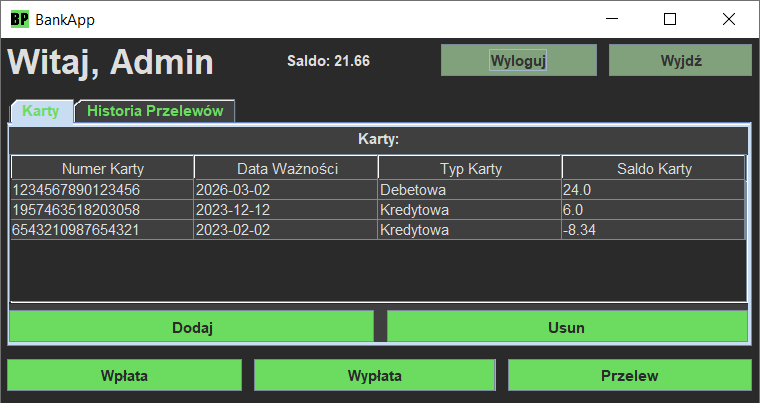
\includegraphics[scale=0.5]{mainkarty}
	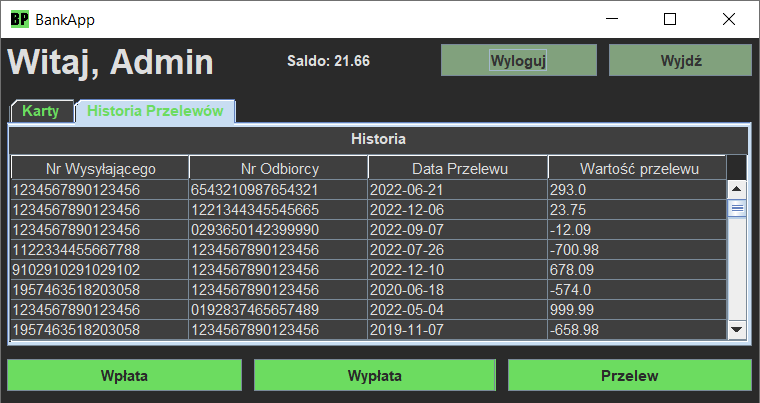
\includegraphics[scale=0.5]{mainhistoria}
\end{center}

\subsection{Dodaj Kartę}

\quad Po wciśnięciu przycisku “Dodaj”, otwiera się okno do dodawania karty.
Składa ono się:

\begin{itemize}
\item Wyboru typu karty (Debetowa/Kredytowa),
\item Nr karty,
\item Przycisku "OK"
\item Przycisku powrotu
\end{itemize}

\quad Aplikacja sprawdza czy nr karty składa się dokładnie z 16 cyfr, i nie zawiera żadnych innych symboli. 
Jeśli dane się zgadzają i użytkownik kliknie przycisk OK, karta zostaje dodana do bazy i okno się zamyka, otwiera się spowrotem główne okno aplikacji.
Natomiast po kliknięciu przycisku powracającego okno się zamyka i otwiera się główne okno aplikacji.

\begin{center}
	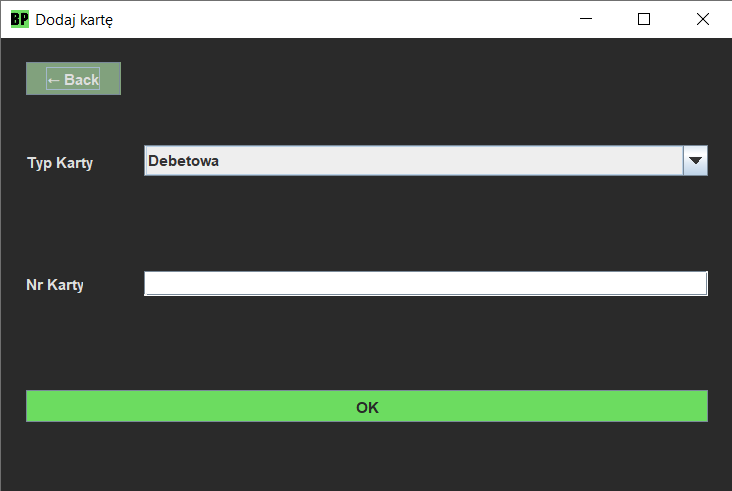
\includegraphics[scale=0.6]{dodaj}
\end{center}

\newpage

\subsection{Usuń Kartę}

\quad Po wciśnięciu przycisku “Usuń” wyświetla się okienko usuwania kart, składających się z:

\begin{itemize}
\item Wyboru karty użytkownika,
\item Typu wybranej karty (Debetowa/Kredytowa),
\item Salda danej karty,
\item Przycisku powracającego,
\item Przycisku "OK"

\quad Po wciśnięciu przycisku OK, aplikacja sprawdzi, czy karta nie zawiera żadnych środków. Jeśli zawiera, zostanie wyświetlony komunikat o braku możliwości usunięcia danej karty. Natomiast jeśli karta jest wyzerowana, zostaje wyświetlone okienko potwierdzania wyboru. Jeśli użytkownik zrezygnuje, wyświetla się odpowiedni komunikat i aplikacja nie wykonuje dalszych operacji. 
Jeśli jednak zaakceptuje to usuwa daną kartę w bazie danych i okno usuwanie jest zamykane.
Po kliknięciu przycisku powracającego okno się zamyka i otwiera się główne okno aplikacji.

\begin{center}
	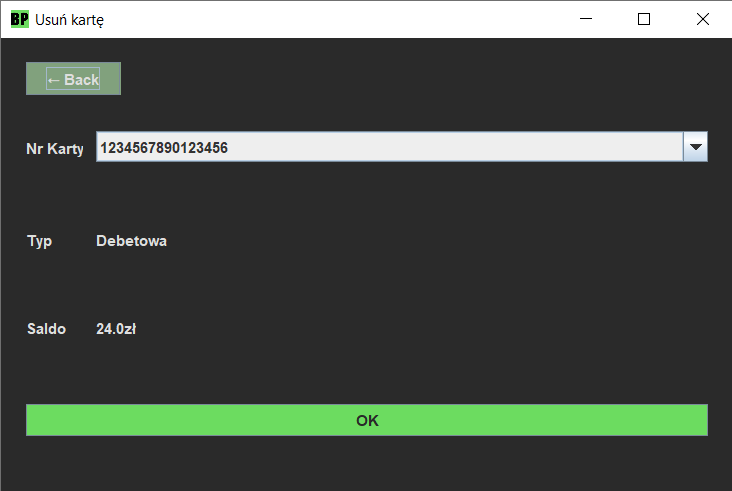
\includegraphics[scale=0.6]{usun}
\end{center}

\end{itemize}

\newpage

\subsection{Wpłata}

\quad Okno wpłaty składa się z:

\begin{itemize}
\item Pola do wprowadzenia wartości wpłacanej kwoty,
\item Pola do wprowadzenia ilości banknotów,
\item Wybór karty na której mamy wpłacić środki,
\item Przycisku "OK",
\item Przycisku powracającego
\end{itemize}

\quad Po wciśnięciu przycisku OK, aplikacja sprawdza:

\begin{itemize}
\item Czy kwota składa się tylko i wyłącznie z liczb,
\item Czy kwota jest większa lub równa 10 i mniejsza lub równa 1000,
\item Czy ilość banknotów jest większa lub równa 1 mniejsza lub równa 10,
\item Jeśli ilość banknotów jest równa 1, to czy kwota jest równa nominałom banknotów (10,20,50,100,200,500)
\end{itemize}

\quad Jeśli walidacja danych przebiegła pomyślnie, kwota zostaje dodana do bilansu danej karty i użytkownik dostaje informację zwrotną wypisującą nr karty i kwotę wpłaconą. 
Jeśli walidacja danych jest błędna, użytkownik zostanie poinformowany, że kwota jest błędna.
Po kliknięciu przycisku powracającego okno się zamyka i otwiera się główne okno aplikacji.

\begin{center}
	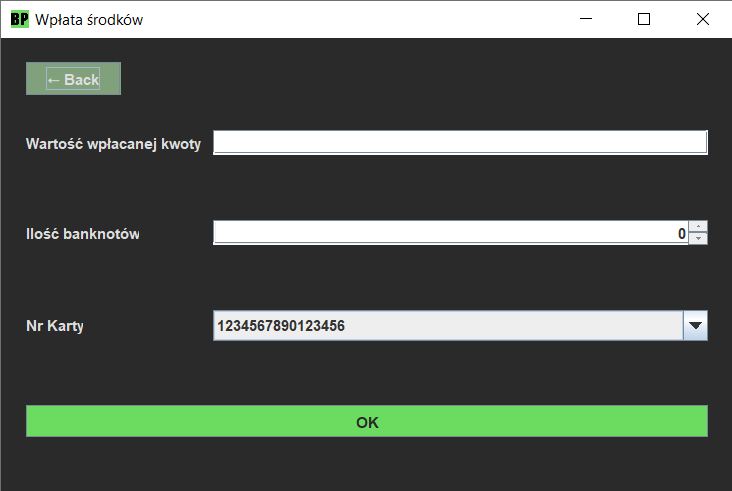
\includegraphics[scale=0.6]{wplata}
\end{center}

\newpage

\subsection{Wypłata}

\quad Po wciśnięciu przycisku wypłaty otwiera się okno zawierające:

\begin{itemize}
\item Wybór karty z której chcemy wypłacić środki,
\item Przycisku typu radio z wartością, jaką chcemy wybrać (50,100,200,300,500,Własna kwota),
\item Pola wprowadzania własnej kwoty, w które możemy wprowadzić dane tylko i wyłącznie jeśli zostanie wybrany przycisk “Własnej kwoty”,
\item Przycisku "OK",
\item Przycisku powracającego
\end{itemize}

\quad Po wciśnięciu przycisku OK program zapisuje kwotę wybraną zależnie od wybranego przycisku. Jeśli użytkownik wybrał własną kwotę, to program sprawdza, czy podał kwotę w polu tekstowym, czy składa się ona wyłącznie z liczb, oraz czy jest większa od 10.
Kwota musi być również podzielna przez 10, ponieważ najmniejszy banknot, który jest możliwy do wydania to banknot 10 zł. 
Jeśli walidacja przeszła pomyślnie, program sprawdza, czy wybrana karta ma wystarczająco środków do wydania kwoty. Jeśli nie, użytkownik zostanie o tym poinformowany. Jeśli tak, to kwota zostaje zabrana z karty i okno się zamyka.
Po kliknięciu przycisku powracającego okno się zamyka i otwiera się główne okno aplikacji.

\begin{center}
	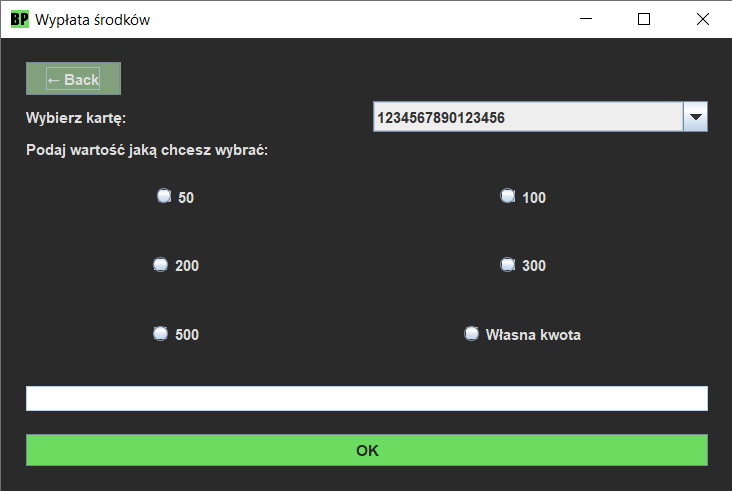
\includegraphics[scale=0.6]{wyplata}
\end{center}

\newpage

\subsection{Przelew}

\quad Po wciśnięciu przycisku wypłaty otwiera się okno zawierające:

\begin{itemize}
\item Wybór karty z której chcemy przelać środki,
\item Pola do wprowadzenia nr karty odbiorcy,
\item Pola wprowadzania kwoty,
\item Przycisku "OK",
\item Przycisku powracającego
\end{itemize}

\quad Po wciśnięciu przycisku OK, aplikacja sprawdza:

\begin{itemize}
\item Czy pole kwoty przelewu nie jest puste?
\item Czy pole odbiorcy przelewu nie jest puste?
\item Czy kwota składa się tylko z liczb?
\item Czy kwota jest większa od 0,?
\item Czy jest wystarczająco środków na danej karcie na przelew?
\end{itemize}

\quad Jeśli walidacja została wykonana pomyślnie użytkownik zostaje poinformowany o pomyślnie wykonanym przelewie o danej wartości na dany nr karty, następnie okno zostaje zamknięte. Dane zostają zapisane do bazy danych. 
Jeśli walidacja nie jest pomyślna, użytkownik zostaje poinformowany o danym błędzie. 
Po kliknięciu przycisku powracającego okno się zamyka i otwiera się główne okno aplikacji.

\begin{center}
	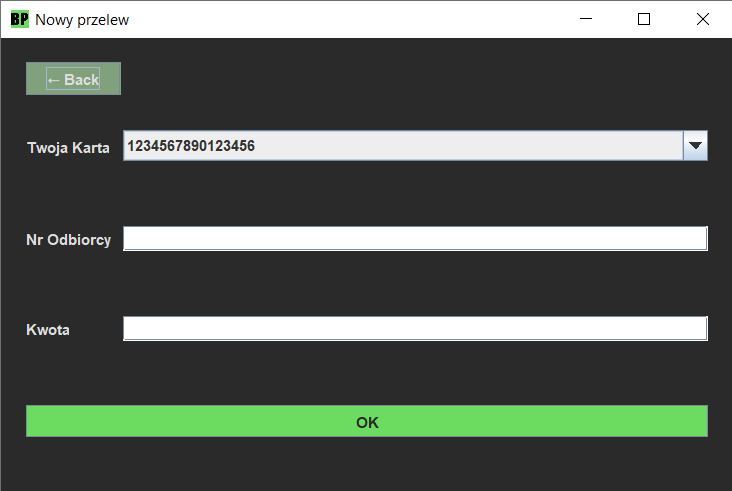
\includegraphics[scale=0.5]{przelew}
\end{center}

\newpage


%--------------------------------------------------------------------------------------------------
%      SYSTEM KONTORLI WERSJI
%--------------------------------------------------------------------------------------------------

\section{System kontroli wersji}

\quad Projekt realizowany był z wykorzystaniem systemu kontroli wersji Git,\\ a wszystkie pliki źródłowe projektu znajdują się pod adresem:\\  \url{https://www.github.com/oskarpasko/BankApp} . 

%--------------------------------------------------------------------------------------------------
%      OPIS TECHNICZNY PROJEKTU
%--------------------------------------------------------------------------------------------------
\section{Opis techniczny projektu}
\begin{itemize}
\item Języki programowania: Java, MySQL
\item Środowiska programistyczne: IntelliJ IDEA, MySQL Workbench
\item Wersja SDK: 18.0.2
\item Aplikacja tworzona na komputery z systemem Windows oraz macOS
\end{itemize}

\newpage

%--------------------------------------------------------------------------------------------------
%      BIBLIOGRAFIA
%--------------------------------------------------------------------------------------------------

\begin{thebibliography}{9}

\bibitem{texbook}
https://www.stackoverflow.com
\bibitem{lamport94}
https://www.codeproject.com

\end{thebibliography}
\end{document}